%A description of your model, with possible reference to one or more sources on which you are building; b. Also, a description of your data source is important…the key variables, the dimensions (i.e., number of x-sectional observations, years included), the extent to which the data are balanced (i.e., the full x-section for each year) or unbalanced (number of missing observations for various years).

The MDP (Manhood Development Program) is a central piece of the African American Male Achievement (AAMA) program. Dee and Penner (2019) already found out that high school dropout rates for black male students can be lowered by the program, and it also has spillover effects on black female students. Therefore, in this paper, I will not specify the sex factor\footnote{What's more, school level data in the EdFacts dataset doesn't have available data for race-sex cells.}.

\noindent My dataset has 321 cross-sectional school level observations over 4 school years: 2011-12, 2013-14, 2015-16, 2017-18. The outcome variable I choose is math percentage of proficiency. This is because to examine the achievement gap, academic outcome would be the best approach. For this key outcome variable, I gathered data from EDFacts data files from the U.S. Department of Education. This database has Mathematics and Reading/Language Arts percentage of proficiency of all schools in the US from grade 3 to high school from SY 2011-12 through SY 2018-19. 

Because of the Family Educational Rights and Privacy Act (FERPA), a Federal law that protects the privacy of student education records, when data is released on groups of students, it can't disclose the individual identity of a student. Therefore, to protect students’ privacy, the US Department of Education used techniques to censor the data for groups that are made up of very few students, since it's easy to identify specific individuals when the sample size is relatively small; or blur the data reported for all other students to further protect the privacy of students and to prevent the possibility that data for small groups being recalculated by subtracting other reported groups data from the reported totals. In order to protect data for small groups, the EdFacts dataset censors all cells with only 1-5 students, and those cells are identified by 'PS'. To blur data for medium-sized groups, EdFacts reports the percentage of proficiency for all medium-sized groups as a range (e.g., $<20\%$ or $70-74\%$). The magnitude of the range is determined by how big the size of the reported group is. For example, cells with 6-15 students (the fewest above the censoring "5 students" cutoff) are reported with the widest ranges like $<50\%$ or $\geq50\%$. The magnitude of the range decreases as the number of students in the reported group increases, until there are more than 300 students in a group, when the percentage of proficiency is reported as a whole number. Since raw data in EDFacts are either 'PS', or all in a form of a range or LE (<=), LT (<), GE (>=), I replace 'PS' with 'NA' and take the mean of the range to make it easier for my analysis. In order to cope with the Civil Rights Data Collection (CRDC)\footnote{Link: https://ocrdata.ed.gov/.} database, which only collects data every second year, I only included SY 2011-12, SY 2013-14, SY 2015-16 and SY 2017-18. 

For the dependent variable, I choose Mathematics percentage of proficiency over that of Reading/Language Arts because interventions usually have a stronger effect on math score than reading score (Cronin, Kingsbury, McCall, and Bowe, 2005). An article from Brookings offers possible explanation: children learn math primarily from school (specifically, in math classes), while they develop reading skills through a broader combination of in-school and out-of-school experiences (Hansen, Levesque, Valant, and Quintero, 2018). However, the different effect of policy impact between Mathematics and Reading/Language Arts is an interesting question and I will compare the different impact of this program on Mathematics scores and Reading/Language Arts scores in a future study.



\noindent My variable of interest is a dummy variable that equals to 1 if a school is in the program in a specific school year, and equals to 0 otherwise. Control variables include out-of-school suspension rate and drop out rate. Out-of-school suspension rate data is collected from the Civil Rights Data Collection (CRDC) database, with school level data including SY 2011-12, SY 2013-14, SY 2015-16 and SY 2017-18. Drop out rate data is collected from DataQuest produced by California Department of Education (CDE). Since drop out rate is only available in high school, I will run regressions for high schools and middle and elementary schools respectively, where the former regression would have two control variables, and the latter would have one control variable. I excluded alternative schools, continuation schools and charter schools.

Table 2 reports summary statistics for the key variables in this study. The gap between black and white math percentage of proficiency is $45.92$ percentage points; when it comes to middle school, the gap became as around $40.06$ percentage points; and for high schoolers, the gap is approximately $34.06$ percentage points. Black Grade 9-12 Dropout Rate is on average $3.2\%$ higher than white Grade 9-12 Dropout Rate. In terms of Out-of School Suspension rate, the difference between black and white students on average is around $8.4\%$. 

\begin{table}[H]
  \begin{center}
    \caption{School Level Descriptive Statistics}
    \label{tab:table1}
    \renewcommand{\arraystretch}{1.5}
    \begin{tabular}{l c c} % <-- Changed to S here.
      \hline
      \textbf{Variable} & \textbf{Mean} & \textbf{Standard Deviation}\\
      \hline
      Black math percentage of proficiency - Elementary school & $35.25\%$ & 24.09\\
      White math percentage of proficiency - Elementary school & $81.16\%$ & 36.56\\
      Black math percentage of proficiency - Middle school & $13.96\%$ & 6.99\\
      White math percentage of proficiency - Middle school & $54.02\%$ & 16.46\\
      Black math percentage of proficiency - High school & $16.58\%$ & 6.55\\
      White math percentage of proficiency - High school & $50.65\%$ & 10.07\\
      Grade 9-12 Dropout Rate - Black & $10.38\%$ & 0.19\\
      Grade 9-12 Dropout Rate - White & $7.16\%$ & 0.17\\
      Out-of School Suspension rate - Black & $12.45\%$ & 0.19\\
      Out-of School Suspension rate - White & $4.02\%$ & 0.11\\
      \hline
    \end{tabular}
  \end{center}
\end{table}

\begin{figure}[H]
  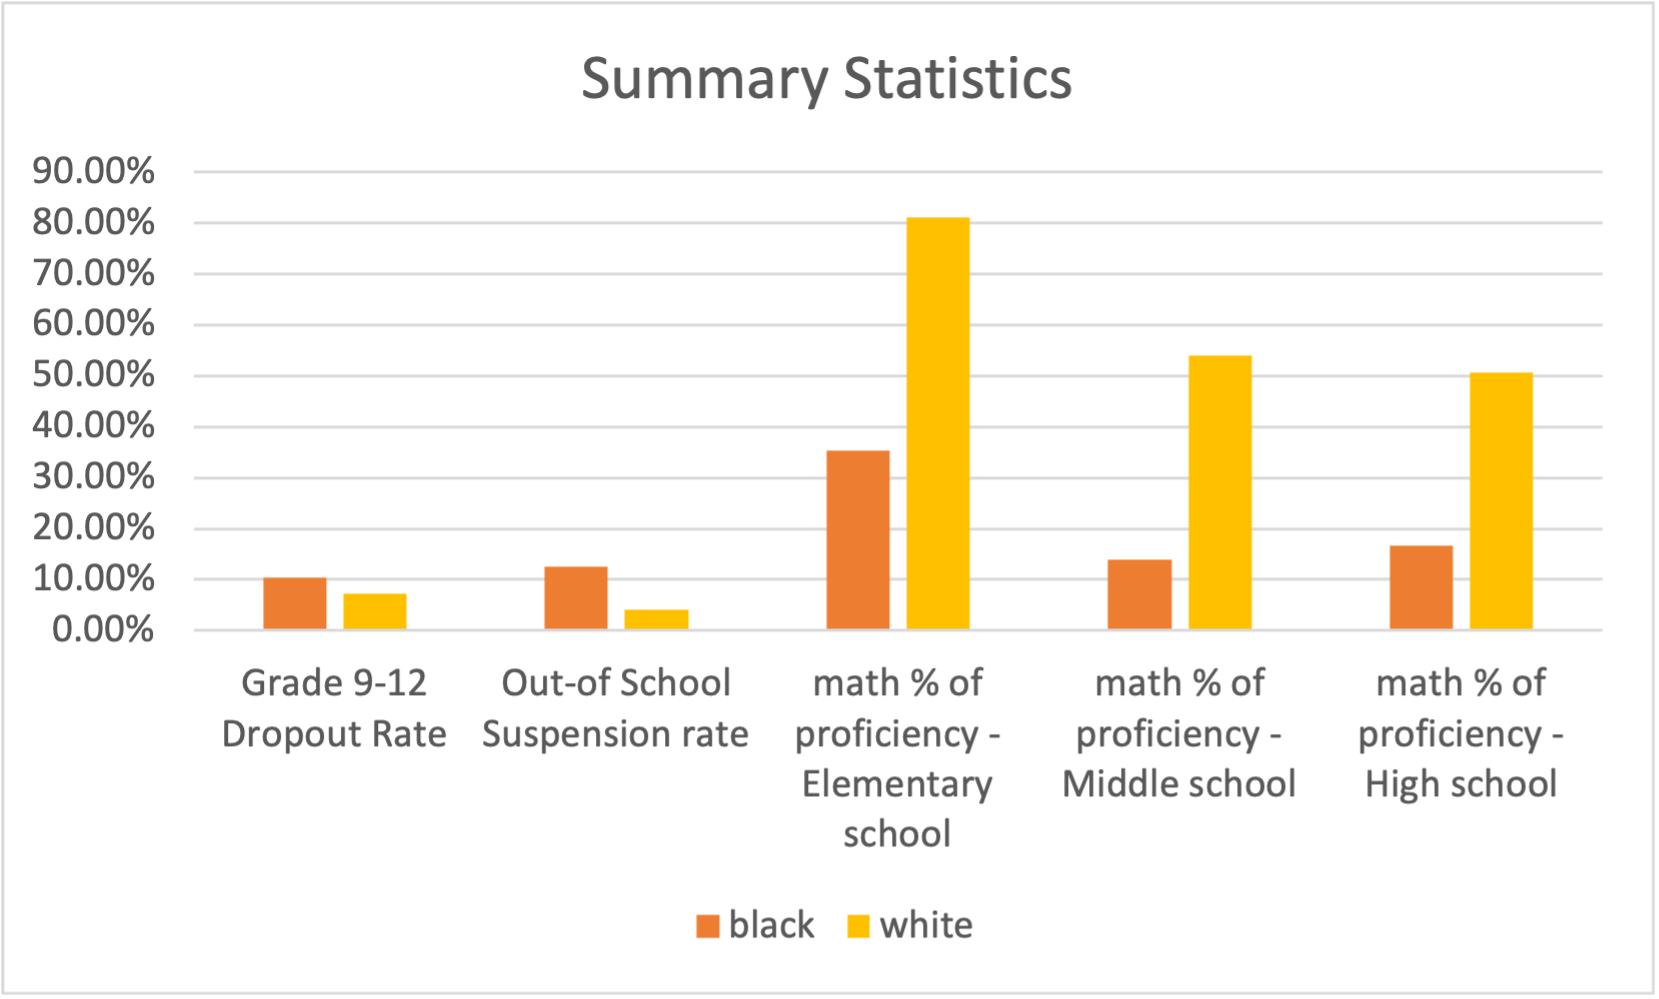
\includegraphics[width=\linewidth]{Picture1.png}
  \caption{Summary Statistics}
  \label{fig:boat1}
\end{figure}

The above figure shows a clearer view of the gap between black and white students in the Oakland Unified School District.

\noindent To realize this, I begin with an OLS specification of the following structure (fixed effects regression):
\[
Y_{st}=\beta_{0}+\beta_1(MDP)_{st}+\beta_2 Z_i+\theta X_{st}+u_{st}
\]
\noindent In the above model, $Y_{st}$ represents the math percentage of proficiency for school cell $s$ in year $t$, and $\beta_{0}$ is the overall intercept. The term, $MDP_{st}$, is a binary variable that stands for whether or not MDP is available at the school in a particular year. $Z_s$ is an unobserved variable that varies from one school to the next but does not change over time. $X_{st}$ represent other control variables that varies both across schools and over time, like drop out rate and out-of-school suspension rate, and $u_{st}$ is an error term.

\noindent Apart from the OLS method, I also report the effect of MDP on the school level using the synthetic control approach as a quasi-experiment evaluate the impact of the program on student academic performance. The synthetic control model I build is referenced from Abadie, Diamond and Hainmueller (2015).

\noindent To start with, I assume that there are $J+1$ units in total, among which $j=1$ is the treated unit, and $j=2$ to $j=J+1$ are potential comparison units (which is often referred to as the "donor pool"). Suppose time periods are represented as follows: $t=1,...,T$. In this case, I assign SY 2011-12 as $t=1$, SY 2013-14 as $t=2$, SY 2015-16 as $t=3$, and SY 2017-18 as $t=4$. I also assume that the sample includes a positive number of pre-intervention periods $T_0$, and a positive number of post-intervention periods $T_1$ where $T=T_0+T_1$. In the OUSD case, although schools didn't launch the program all at the same time, the window was very close. So I take SY 2013-14 as $T_0+1$ for high schools and SY 2015-16 as $T_0+1$ for elementary schools and middle schools. By assumption, $j=1$ is only exposed to the treatment in periods $T_0+1,...,T$ and units $j=2$ to $j=J+1$ receive no treatment at all whatsoever. 

\noindent After identifying basic definitions, I define a synthetic control as a weighted average of units in the comparison group. In other words, the synthetic control can be represented by a weight vector
\[
W=(w_2,...,w_{J+1})
\]
where 
\[
0\leq w_j\leq 1~for~j=2,...,J~and~w_2+...+w_{J+1}=1.
\]
Here, a synthetic control is equivalent to a particular value for $W$. Therefore, I need to find the value of $W$ that is closest to the characteristics of the treated unit during the pre-intervention period. Call $X_1$ as a $(k\times 1)$ vector that contains values of the characteristics of the treated unit pre-intervention. Now, suppose $X_0$, a $(k\times J)$ matrix, collects values of the same variables for units in the comparison group. I want to select the synthetic control $W^*$ that minimizes the difference between the pre-intervention characteristics of the treated unit and the synthetic control $X_1-X_0W$.

\noindent This can be realized as follows: let $X_{1n}$ be the value of the $n$-th variable of the treated unit and $X_{0n}$ be a $(1\times J)$ vector composed of values of the $n$-th variable of the comparison unit (i.e., the donor pool). Choose $W^*$ as the value of $W$ that minimizes
\[
\sum^k_{n=1}v_n(X_{1n}-X_{0n}W)^2,
\]
where $v_n$ is a weight that reflects the relative importance level of the $n$-th variable when measuring the difference between $X_1$ and $X_0W$.

\noindent With that, I can predict the effect of the program by comparing characteristics of the treated unit and the synthetic control post intervention. Define $Y_{st}$ as the outcome of unit $s$ at time $t$. Suppose $Y_1=(Y_{1T_0+1},...,Y_{1T})$ is a $(T_1\times 1)$ vector that collects post-intervention values of the outcome for the treated unit, and $Y_0$ is a $(T_1\times S)$ matrix where column $s$ contains the post-intervention values of the outcome for unit $s+1$. For the post-intervention period $t$, where $t\geq T_0$, the effect of the treatment is estimated by the synthetic control as the disparity between the outcome of the treated unit and the outcome of the synthetic control:
\[
Y_{1t}-\sum^{S+1}_{s=2}w_s^*Y_{st}.
\]

